%!TEX root = Main.tex
%\section{Limitations and future work}
%\vspace{-0.1in}
%\subsection{Limitations and future work}

%\textbf{Mid-connection mobility:} In this paper, we have focused on reducing the time-to-connect through the global name service. However, a complete solution needs to also support mid-connection mobility, especially simultaneous mobility of both endpoints (as the mobility of just one endpoint can be handled bilaterally without relying on the global name service). We have developed a user-level socket library, \verb+msocket+, that enables application developers to seamlessly develop network applications using \auspice\ at connection initiation time, using bilateral connection migration for individual mobility, and falling back on \auspice\ to handle simultaneous mobility. Under simultaneous mobility, we have shown that endpoints can re-establish a connection within $\approx$2RTTs of the latter endpoint coming back online. However, a detailed description of \verb+msocket+ is nontrivial and is described in a separate report \cite{msocket}.

%\textbf{Future workloads:} The design of \auspice\ is primarily motivated by high mobility or high update rates that we take for granted, but we do not know what a future mobile lookup workload might look like. In the absence of a definitive workload, we have shown that \auspice\ offers significant cost-benefit tradeoffs for a broad range of projected mobile workloads as well as for today's largely non-mobile domain names. 

%\textbf{Scope of evaluation:} Our comparison of \auspice\ to managed DNS providers pits a pre-release prototype against opaque production services in live operation, an admittedly narrow comparison. Furthermore, we stand on loose footing with prototype-driven experiments involving $10^4$ names and simulation experiments involving $10^6$ names against DNS that serves $10^8$ names and commands the luxury of decades of deployment experience, so our contribution is but academic at this point.

%- msocket. Critical to show mid-connection mobility. We have shown proof-of-concept that endpoints can recover from simultaneous mobility within 2 RTTs of the latter client coming back online. A detailed design and implementation appears in a separate paper.

%- we do not have a reasonable way to predict mobile workloads of the future. Best we can do is sensitivity analysis of key workload parameters.

%- comparing absolute numbers with a prototype with production managed DNS services is unfair. However, we do not have sufficient exposure into internal proprietary design details.

%- geolocation-based distance is not network distance.

%\textbf{Estimating network distances:} \auspice's placement engine relies on efficiently estimating network distances based on the network addresses of clients or local name servers. Our current implementation involves infrequently measuring ping latencies between name servers and local name servers; as part of ongoing work, we are evaluating  other alternatives including using IP-to-geo distances or iPlane \cite{iplane} in conjunction with EDNS \cite{EDNS} options to efficiently estimate network distances to both local name servers and originating end-hosts.

\eat {
	\textbf{Deployment:}  We discuss deployment possibilities of \auspice\ in a multi-provider scenario, unlike the single provider scenario described earlier in the paper. Existence of multiple providers of \auspice\ would foster competition resulting in better quality of service, and would give a customer the freedom to choose the provider she considers most trustworthy. 
	
	To resolve a name X to its address in the presence of multiple providers, a client first needs to \emph{pre-resolve} X to its \auspice\ provider P. Pre-resolving a name is trivial in the special case when names are structured and a fixed part of name identifies its provider, e.g.. all names of the provider ``microsoft'' are of the form ``microsoft.userXYZ''. In general,  for a flat name X, the pre-resolution can be achieved by a federated DHT across the set of \auspice\ providers. The result of the pre-resolution, i.e., the tuple [X, P], can be cached by any intermediary or endpoint as \auspice\ providers are expected to change infrequently. 
	The task of resolving names to \auspice\ providers may seem similar to that of resolving names to addresses. However, the former is an easier problem because the
	update costs associated with storing name-to-\auspice\ provider mappings are much smaller. 
}
%  \auspice\ provider for a name is expected to change much more slowly than its address. Hence, update costs for storing name-to-\auspice\ provider mappings are much smaller.

%The pre-resolution may be facilitated by a local name server and the tuple [X,P] can be cached by any intermediary or endpoint as \auspice\ providers are expected to change infrequently. 



%A special case is that of structured names as in DNS. 
%
%Due to the small update costs, 
%
%name to auspice \auspice\ mapping are expected to change at much smaller rates 
%
%. This is because name to \auspice\ provider mappings are expected to change infrequently 



%To resolve a flat name X, endpoints must first {\em pre-resolve} X to its GNS provider P. This pre-resolution may be facilitated by a local name server and the tuple [X,P] can be cached by any intermediary or endpoint as GNS providers are expected to change infrequently. The pre-resolution can be achieved either by explicitly querying all GNS providers if they are small in number (as we expect) or as a federated DHT across the set of GNS providers.  Our primary focus is on the design of an individual GNS provider (like P) that must rapidly translate names of its endpoint customers (like X) to their network addresses. 

%
%Our envisioned global name service (GNS) architecture must translate names of mobile endpoints to their  addresses with the following qualitative design goals.
%
%
%{\bf (1) Arbitrary names}: The design must must not enforce a specific naming structure, e.g., www.yahoo.com or XYZ3142.google or /microsoft/user2178, allowing them to be flat, i.e., arbitrary strings of bounded length. Structured names either inevitably lead to assumptions about restricted mobility or result in endpoint names that change as they move, requiring an additional infrastructure to resolve a canonical name to a temporary name. In comparison, flat names can enable intrinsic support for authentication if defined in a self-certifying manner (as in HIP\cite{HIP} and follow-ons \cite{AIP,MobilityFirst,AIP}).
%
%{\bf (2) Federated deployability}: The deign must enable federated deployment, i.e., a single organization must not be responsible for providing name service to all names, for scalability and trustworthiness. DNS does satisfy this design goal by delegating portions of a hierarchical name space to different organizations, but does so by mandating structured names.
%
%{\bf (3) User choice}: The design must allow for multiple GNS providers to co-exist and compete and for endpoints to freely choose their GNS provider, similar in spirit to how domains today can choose authoritative DNS service managed by third-parties. This requirement precludes DHT-based designs that assign responsibility for managing a name's resource records to a randomly chosen infrastructure node (as in CoDoNS\cite{codons-paper}).
%


%\begin{figure}[t]
%\centering
%
%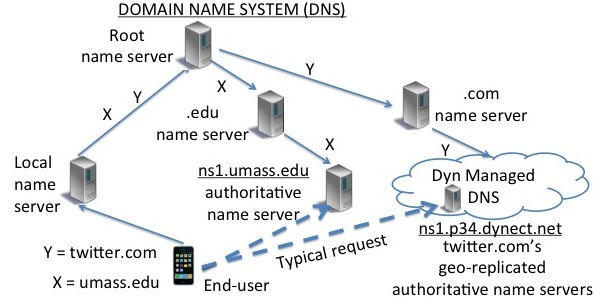
\includegraphics[scale=0.4]{gns-dns/Slide1.jpg}
%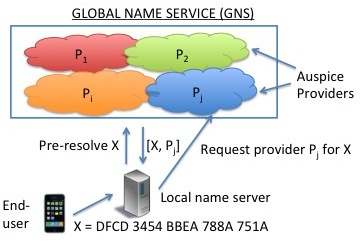
\includegraphics[scale=0.5]{gns-dns/Slide2.jpg}
%\vspace{-0.2in}
%\caption{Top: Hierarchical name resolution in DNS. Bottom: Proposed GNS architecture for resolving arbitrary names to network locations.}
%\vspace{-0.2in}
%\label{fig:DNS_GNS}
%\end{figure}



%Figure \ref{fig:DNS_GNS} illustrates our envisioned GNS architecture contrasting it with the current DNS. To resolve a flat name X, endpoints must first {\em pre-resolve} X to its GNS provider P. This pre-resolution may be facilitated by a local name server and the tuple [X,P] can be cached by any intermediary or endpoint as GNS providers are expected to change infrequently. The pre-resolution can be achieved either by explicitly querying all GNS providers if they are small in number (as we expect) or as a federated DHT across the set of GNS providers.  Our primary focus is on the design of an individual GNS provider (like P) that must rapidly translate names of its endpoint customers (like X) to their network addresses. 


\eat{
	\textbf{Security:}
	
	\textbf{Mid-session mobility:}
	
	\textbf{Paxos overhead:}
}
\vspace{-0.1in}
\section{Related work}
\label{sec:related}

%To our knowledge, this is the first paper to study the problem of locality-aware service replica placement and use the insights to drive the design and implementation of a global name service. Nevertheless, an enormous body of prior research has studied naming, server selection, and placement issues in large-scale distributed systems, as discussed below.

Our work draws on lessons learned from an enormous body of prior work on network architecture as well as distributed systems, as described in Section \ref{ch:intro-auspice} and Section \ref{sec:bg}. We discuss related work not covered elsewhere in the paper here.

%Compared to the former, the novel contribution in \auspice\ is an engine to {automate} geo-distributed replica placement to achieve low-latency, low-cost, and high availability.  Compared to the latter, our contribution is a global name service with intrinsic support for mobility for the Internet as well as ``future'' Internet or endpoint architectures such as MobilityFirst, XIA, or HIP.
%in a low-cost, locality- and load-aware manner.

%\textbf{DNS:} Until the early 80s, the Internet relied on a system called \verb+HOSTS.TXT+ for name resolution, which was simply a centrally maintained text file distributed to all hosts. The current Internet's distributed DNS \cite{DNS} arose in response to the rapidly increasing size of the file and the cost of distributing it. Mockapetris and Dunlap point to TTL-based caching to reduce load and response times as a key strength, noting that ``{\em the XEROX system {\em [Grapevine \cite{grapevine}]} was then ... the most sophisticated name service in existence, but it was not clear that its heavy use of replication, light use of caching ... were appropriate}''. We have since come a full circle, turning to  active replication in \auspice\ in order to address the challenges of mobility, a concern that wasn't particularly pressing  in the 80s. Compared to classical systems like Grapevine or ClearingHouse, \auspice\ enables support for automated demand-aware replica placement for arbitrary names; it also differs in several basic elements such as the use of Paxos, the key-value abstraction, self-certifying names, consistent hashing etc., that were not known back then.  \auspice, through its support for context-aware delivery, is also a step towards addressing some of the challenges to which Lampson alludes on representing ``descriptive names" \cite{Lampson}.

%\textbf{DNS enhancements:} 
%Since then, 
{\bf{DNS:}} Many have studied issues related to performance, scalability, load balancing, or denial-of-service vulnerabilities in DNS's resolution infrastructure \cite{Pappas,codons-paper,Brownlee,dnssec}. Several DHT-based alternatives have been put forward \cite{codons-paper,cox,DHTdns} and we compare against one representative proposal, Codons \cite{codons-paper}. In general, DHT-based designs are ideal for balancing load across servers, but are less well-suited to scenarios with a large number of service replicas that have to coordinate upon updates, and are at odds with scenarios requiring placement of replicas close to pocket of demand. In comparison, \auspice\ uses a planned placement approach.

Vu et al. describe DMap \cite{VuICDCS12}, an in-network DHT scheme %to map a self-certifying identifier to a fixed number of resolver locations using different consistent hash functions with clients choosing the closest mapped resolver. This approach 
that is similar in spirit to \staticthree\ as evaluated in our experiments (Section \ref{sec:eval}) (with a more direct comparison in \cite{techreport}), showing that demand-aware placement can dramatically outperform randomized placement. A more important qualitative distinction is that DMap ties federation to the interconnection structure between ISPs, which entails commensurate lookup latency penalties and potential incentive mismatches by mapping GUIDs to non-provider ISPs. In comparison, the \auspice\ approach decouples the federation structure between GNS providers from that between ISPs.


%In contrast, our work targets scenarios with potentially high update rates and seeks to place replicas to achieve low-latency, low-cost and high availability.

%Classic works on name services such as Grapevine and others \cite{XeroxClearingHouse, LampsonPODC86} for distributed resource discovery have influenced a number of more recent works such as the Intentional Naming System\cite{INS} and Active Names\cite{ActiveNames} that have several orthogonal goals compared to \auspice.
%INS\cite{INS} proposes a naming system that is also in large part motivated by mobility, but unlike INS that emphasizes expressiveness of {\em intentional} names, one of our goals is to resolve unique but verifiable identifiers. Furthermore, replication, low-latency and low-cost placement of name records, or wide-area interdomain environments are not targeted by INS.  Active Names allows applications to deploy mobile code at resolvers that can recursively invoke other programs for finer-grained, hierarchical resolution and compose the output of resolved services. In contrast, \auspice\ does not attempt to support mobile code or service composition, but does supports the resolution of identifiers to other identifiers before eventual resolution to network locations. As part of ongoing work, we are exploring adding support for active resolution objects \cite{comet} in \auspice.


%Classic works on name services such as Grapevine and others \cite{XeroxClearingHouse, LampsonPODC86} for distributed resource discovery have influenced a number of more recent works such as the Intentional Naming System\cite{INS} and Active Names\cite{ActiveNames}. INS\cite{INS} proposes a naming system that is also in large part motivated by mobility but has several orthogonal goals. INS allows clients to specify their intention as opposed to a unique name in a simple, high-level language, and the resolution overlay network is tightly integrated with routing, thereby enabling late-binding of intentions to matching destinations. Unlike INS that emphasizes expressiveness of names but not security, one of our goals is to resolve unique but verifiable identifiers. Furthermore, replication, locality-aware placement of resolvers, or wide-area interdomain environments are not targeted by INS. 

%Active Names allows applications to deploy mobile code at resolvers that can recursively invoke other programs for finer-grained, hierarchical resolution and compose the output of resolved services. In contrast, \auspice\ does not support mobile code and does not attempt to support service composition, but does supports the resolution of identifiers to other identifiers (e.g., for geocast) before eventual resolution to network locations. As part of ongoing work, we are exploring adding support for active resolution objects \cite{comet} in \auspice.

\textbf{Request redirection:} Many prior systems have addressed the request redirection problem with data or services replicated across a wide-area network as discussed in the context of CDNs in Chapter \ref{ch:te-background}. Examples include anycast services \cite{oasis,Bhattacharjee:1997:AA:839292.843045,donar} to map users to the best server based on server load or network path characteristics. These systems as well as CDNs and cloud hosting providers share our goals of proximate request redirection and load balance given a fixed placement of server replicas. \auspice\ differs in that it additionally considers replica placement itself as a degree of freedom in achieving low latency or load balance.

\textbf{Dynamic placement:} We were unable to find prior systems that {\em automatically} reconfigure the {\em geo-distributed} replica locations of frequently {\em mutable objects} while preserving {\em consistency} (i.e., those satisfying all four italicized properties). However, reconfigurable placement has been studied for static or slow changing content \cite{gwertzman:95b} or within a single datacenter, or without replication. For example, Volley \cite{volley} optimizes the placement of mutable data objects based on the geo-distribution of accesses and is similar in spirit to \auspice\ in this respect, however it implicitly assumes a single replica for each object, so it does not have to worry about high update rates or replica coordination overhead. %As shown in  Section \ref{sec:eval}, creating multiple replicas of objects or services can significantly reduce user-perceived response times while also enhancing opportunities to balance load provided update cost is taken into account.
%\auspice\ is also similar in spirit to edge services hosted by CDNs. However, unlike \auspice, the geo-distributed locations of edge services as well as cloud-hosted services today are chosen manually and infrequently updated. %In comparison, \auspice\ automates geo-distributed placement of replicas, but the ``service'', a key-value store, is much simpler compared to black-box cloud-hosted services.


%CDNs dynamically cache copies of static content near points of demand. In comparison, \auspice\ makes active replicas of dynamic objects (or name records) in a planned manner. Planned placement is typically considered unnecessary for static content distribution as simple caching and replacement schemes suffice to capture most of the benefit\cite{DoWeNeedReplica,NCDN}. \auspice\ is closer in spirit to edge services offered by commercial CDNs. However, the geo-distributed locations of edge services as well as cloud-hosted services today are chosen manually and infrequently updated. In comparison, \auspice\ automates geo-distributed placement of service replicas, but the service, name resolution, is much simpler compared to black-box cloud-hosted services.



%Sandpiper \cite{sandpiper} optimizes the placement of virtual machines in order to mitigate hotspots at physical machines within a datacenter. The approach infers the utilization levels of multiple resources at each physical machine by monitoring queueing delays or by direct measurement when feasible and live-migrates VMs from heavily loaded physical machines to lightly loaded ones.  Other systems \cite{TimWood,VahdatOSDI} have shown that placing VMs cleverly on physical machines can improve performance because of sharing memory pages. Unlike \auspice, the placement decisions in these systems do not significantly impact user-perceived response times as they are within a local area network, and do not explicitly address replication or update cost, but are designed for more general services than name name resolution.

%Theoretical works have studied many variants of facility location location problems that, like the formulation in Section \\ref{sec:design}, are in general computationally hard. Some facility location problems lend themselves to efficient approximation algorithms \cite{facilitylocationapprox}. It is unclear if the formulations in Section \\ref{sec:design} allow for efficient approximation algorithms and it is part of ongoing work to develop approximation algorithms that lend themselves to an uncoordinated implementation across the hosted services.

\auspice\ is related to many distributed key-value stores \cite{mongodb,Escriva,cassandra}, most of which are optimized for distribution within, not across, data centers. Some (e.g., Cassandra) support a geo-distributed deployment using a fixed number of replica sites. Spanner \cite{spanner} is a geo-distributed data store that synchronously replicates data (``directories'') across datacenters with a semi-relational database abstraction. Compared to Spanner, \auspice\ does not provide any guarantees on operations spanning multiple records, but unlike Spanner's geographic placement of replicas that  ``administrators control'' by creating a ``menu of named options'',  \auspice\  automatically reconfigures the number and placement of replicas so as to reduce lookup latency and update cost. Furthermore, Spanner assigns a large number of directory objects to a much smaller number of fixed Paxos groups; \auspice\ supports an arbitrarily reconfigurable Paxos group per object based on principles in recent theoretical work on reconfigurable consensus, e.g., Vertical Paxos \cite{vertical-paxos} and the more recent report on Viewstamped Replication Revisited \cite{liskov12vr}.

%Spanner provides database like features, e.g., distributed transactions, 
%implements general purpose database features such as distributed transactions for globally replicated data. \auspice\ provides limited support for operations spanning multiple records, its primary focus is to automatically determine placement of 


%TBD: Other DNS enhancements, e.g., piggybacking domain names, and non-DHT architectures?

%\textbf{XIA:} Like MobilityFirst, the XIA future Internet architecture \cite{XIA} also uses self-certifying identifiers and network locations. Self-certifying identifiers are not new and have been used in a variety of distributed systems \cite{Mazieres,BitTorrent} as well as  specifically in the context of Internet architecture \cite{AIP,DONA}. In both XIA and MobilityFirst, a self-certifying identifier can be used to represent a variety of principals. For evolvability, XIA represents addresses as a directed acyclic graph of self-certifying identifiers. Paths in this graph correspond to possible ``source routes'' to reach the destination, but not all routers need be capable of processing every identifier and could instead fallback to the default address of the form [GUID, NA]. In comparison, MobilityFirst is designed with more explicit support for mobility-centric services while keeping addresses and packet headers simple. Evolvability comes from the support for indirection and grouping in the global name resolution service that can resolve a GUID to a set of one or more GUIDs. 


%TBD: discuss authoritative name servers or lack thereof somewhere.

%\textbf{Geo-distributed clouds:} TBD: Not sure what we have to say about them here. Just place a list of these references earlier: PlanetLab \cite{planetlab},  Akamai Edge Computing \cite{edgecomputing}, Amazon EC2 \cite{amazonec2}, Google app engine \cite{google-app-engine}, Windows Azure \cite{windowsazure}.

\eat {
	\textbf{DNS:}
	
	- CODONS \cite{codons}
	
	- Design and Implementation of an Intentional Naming System
	
	- A comparative study of the DNS design with DHT-based alternatives
	
	- Piggybacking related domain names to improve DNS performance
}

\eat {
	- OASIS: Maps users based on IP addresses to best server by comparing latency and server load. \cite{oasis}
	
	- ClosestNode:  An open access, scalable, shared geocast service for distributed systems.
	
	- DONAR: Provides customization of mapping policies for various content providers. \cite{donar}
	
	Our primary contribution is a system that automatically decides server placement considering popularity and geographic distribution of requests. 
}

\eat {
	\textbf{VM Placement:}
	
	- Sandpiper: solves VM placement problem \cite{sandpiper}
	
	\textbf{Data Placement:}
	
	
	Placement for static data: 
	
	- Do We Need Replica Placement Algorithms in Content Delivery Networks?
	
	- Constrained Mirror Placement on the Internet
	
	- Optimal Content Placement for a Large-Scale VoD System
	
	Placement for dynamic data: 
	
	- Volley. \cite{volley}
}


%- Approximation algorithms for facility location problems. \cite{facilitylocationapprox}






